\section{Mechanics} \label{sec:mech}

\subsection{Requirements}

% ===== Relation to System Level Requirements ===== %
The mechanical part should be constructed such that:
\begin{itemize}
    \item There must be enough space for electronic components to fit in.
    \item Camera unit should be adjusted properly so that it should be protected from animal attacks.
    \item There must be no obstacle in front of the camera unit, so that it can capture accurate photographs.
    \item Angle and the position of the camera must be adjusted properly in order to identify cats and dogs from 1.5 meter.
    \item Integration of the food mechanism should be such that it must waste minimum amount of food, and the food given to the cats must be controllable in terms of the quantity.
    \item Capacity of the reservoir should be 4 kg (in full capacity) in order to provide 150 meals for a standard cat.
    \item Unwanted dogs must be deterred without giving harm.
    \item Amount of food remaining, battery chargers while loading and in operation should be visible by the user easily.
    % USER OLMAMIS SANKI, USER ONLY WHEN DESIRED FALAN OLABILIR.
    \item Overall system must be resistant to heat and cold. It must be waterproof, and sturdy. Most importantly the weight of the overall system should be around 10 kg so that it can be carried by a single person.
\end{itemize}

Mechanical design is composed of two parts: 
\begin{itemize}
    \item The interior design
    \item The exterior design
\end{itemize}

In the interior design there exit several parts like:
\begin{itemize}
    \item Inner cable connections is done.
    \item Food mechanism is placed.
    \item Reservoir and the electronic components are fitted into the box.
    \item Integration of the dog deterring system will be done. 
\end{itemize}
Connections will be done properly since every extra cable creates a clutter inside the system. The electronic components will be placed as close as possible in order to shorten the cables length. There will be minimum number of cable between the flowing food in order not to block the food flow and to protect the hygiene of the food. 

Food mechanism will be stable and sturdy. It will be fixed between the food reservoir and the path that food will flow. The details of the food mechanism will be discussed in the below for the mechanical part of this report.

Dog deterring system must annoy dogs and deter them from the area without causing them harm. The details about the system can be found in the subsystems and risks part.

The exterior design is mostly composed of the durability of the case. Its sub-parts can be observed below.
\begin{itemize}
    \item Camera will be mounted properly.
    \item Material for outer design should be selected such that it must be economic, durable and must not exceed 6 kg for all outer design.
\end{itemize}

The expected size of the box is 40X26X50 $cm^{3}$ with maximum 10 kg weight.

% ===== Indicate alternative solutions ===== %
\subsubsection{Food Mechanism}
 Food mechanism should contain four important features:
\begin{itemize}
    \item The food flow must be controllable.
    \item Power consumption should be low in order to sustain 5 hours of non-stop working.
    \item Minimum amount of food should be wasted.
    \item Weight of the overall food mechanism (reservoir and motor together) should not exceed 5 kg.
\end{itemize}
In order to satisfy these four conditions, two different solution plans are considered.
\paragraph{Part A}
In order to control the flow amount, it is considered that first storing nearly 30 gr of food in an empty area, then by pouring this stored food, we planned to control the quantity of the food given. To do so a 45mm radius cylinder (4.5 mm depth) shaped apparatus will be used. \%25 of the cylinder is empty and free to store food. The cylinder is between the reservoir and the obstacle that cuts the food flow. The food will be first poured to the empty region of the cylinder due to the gravity, then it will be stored there until a cat arrives. When a cat arrives the servo motor (MG99R which has 9.4 kg-cm torque) rotates the cylinder. The stored food in the empty region of the cylinder rotates through the pour free region of the obstacle and will be poured down when it reaches an opening. By this way in every two rotation of the cylinder 15 gr of food is supplied to the cat. The technical drawing of the cylinder can be seen from the figure~\ref{fig:cylinder}.

\begin{figure}[ht]
     \centering
     \begin{subfigure}[b]{0.49\linewidth}
     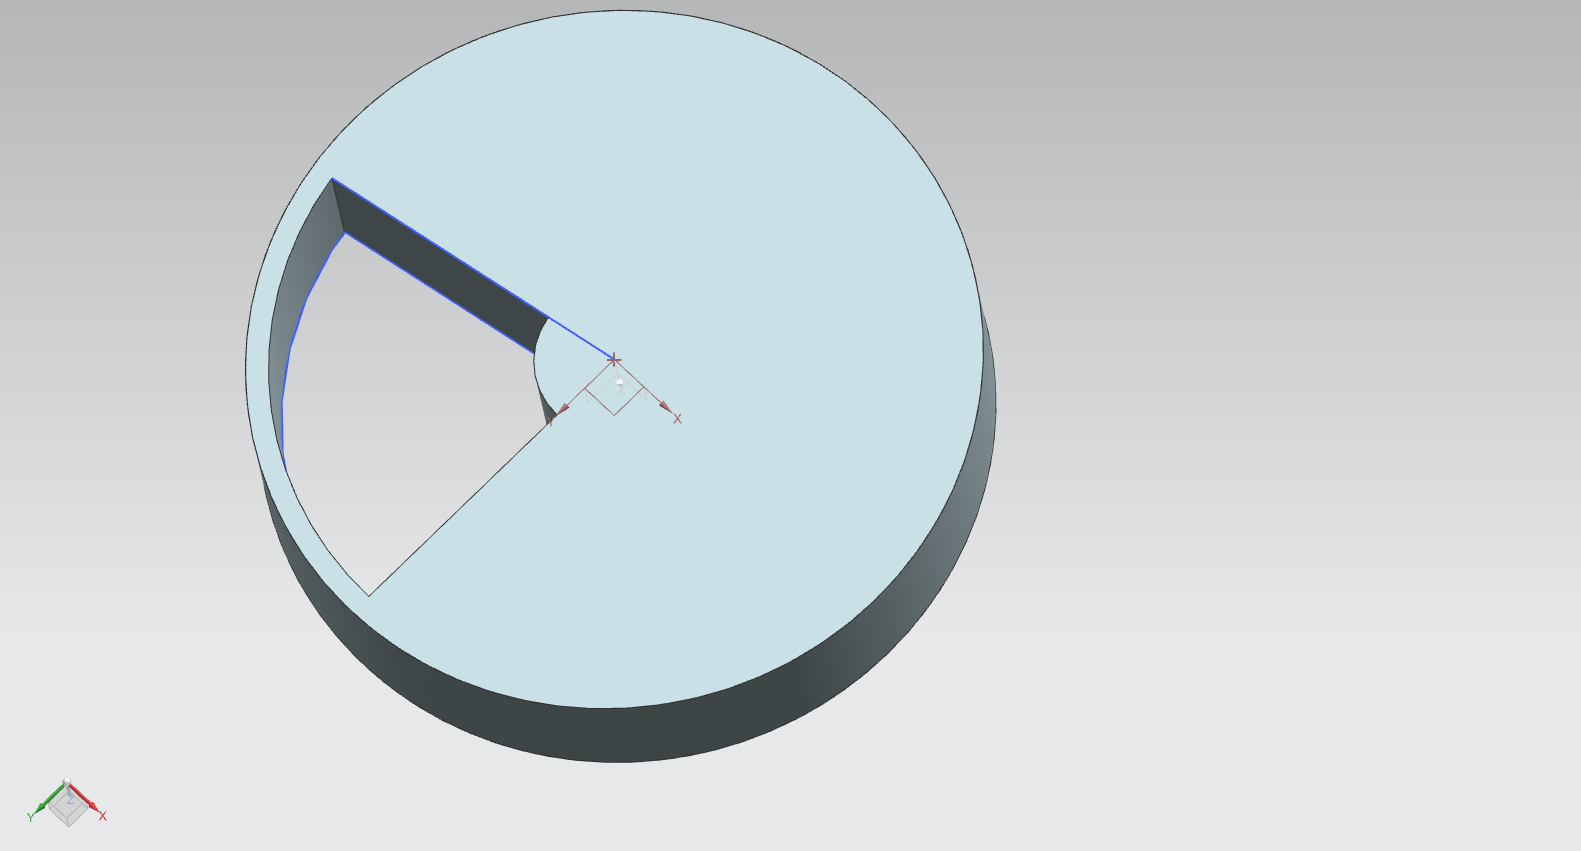
\includegraphics[width=\linewidth]{img/cylinder.png}
     \caption{Cylinder}
     \label{fig:Cylinder1}
     \end{subfigure}
     \begin{subfigure}[b]{0.49\linewidth}
     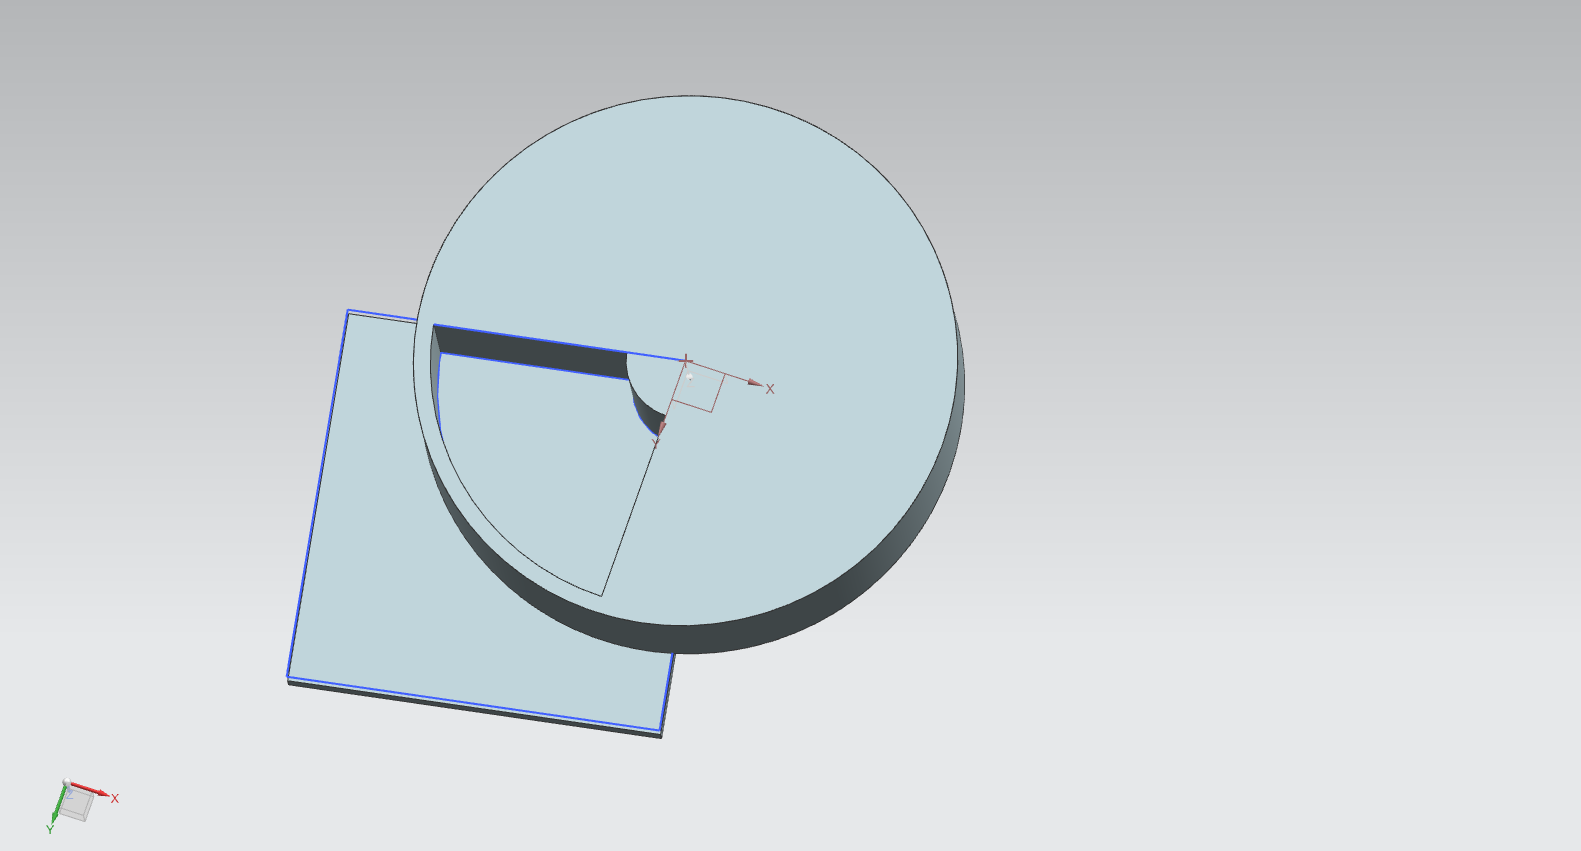
\includegraphics[width=\linewidth]{img/cylinder2.png}
     \caption {Cylinder in Off state}
     \label{fig:Cylinder2}
     \end{subfigure}
     \label{fig:pwm}
     \begin{subfigure}[c]{0.49\linewidth}
     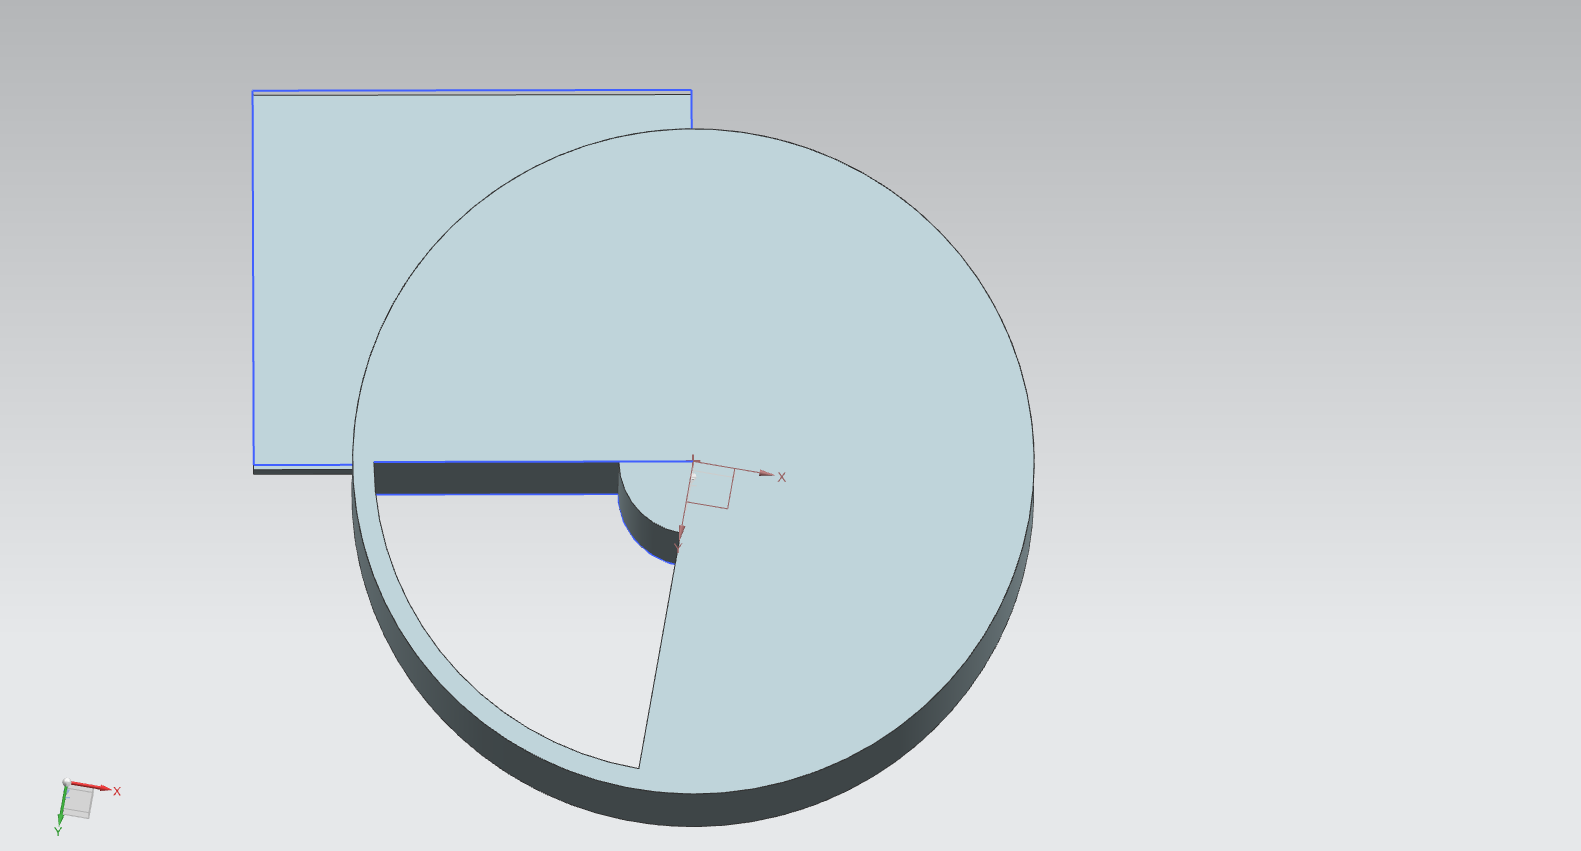
\includegraphics[width=\linewidth]{img/cylinder3.png}
     \caption {Cylinder in On state}
     \label{fig:Cylinder3}
     \end{subfigure}
     \caption{The representation of the disk}
     \label{fig:cylinder}
\end{figure}

% ASUDEYE NOT: ASAGIDAKI PARAGRAFA TEKRAR BAk. 
When food is pouring from the cylinder also the food in the reservoir will also flow on to the cylinder due to the gravity, however, they will be stopped by the solid part of the cylinder and by this way the food flow from the reservoir will be stopped. There are still considerations if this design will properly stop the food, therefore there exist a plan B

\paragraph{Plan B}

This plan mainly considers stopping the food flow. There will be two identical disks which their radius is 45mm. One-third of these disks are empty. One of them can rotate and other can't. The stable disk is connected to the end of the reservoir and the other one is placed right under the stable disk. Servo motor is connected to the rotating free disk and the motor provides the necessary torque (12 kg-cm) to rotate it. When two open sides are matched, the food stars to flow through the empty region, and when one opens and one closed side is matched the food flow stops.  
This solution is a practical way to stop the food flow when there is no cat however, it is problematic in terms of the controlling the quantity of the food. Moreover there exist some other problems like what will happen when a food is jammed between the reservoir and disk. one can see the representation of the disks from the Figure~\ref{fig:Disk}.
\clearpage 

\begin{figure}[t!]
     \centering
     \begin{subfigure}[b]{0.49\linewidth}
     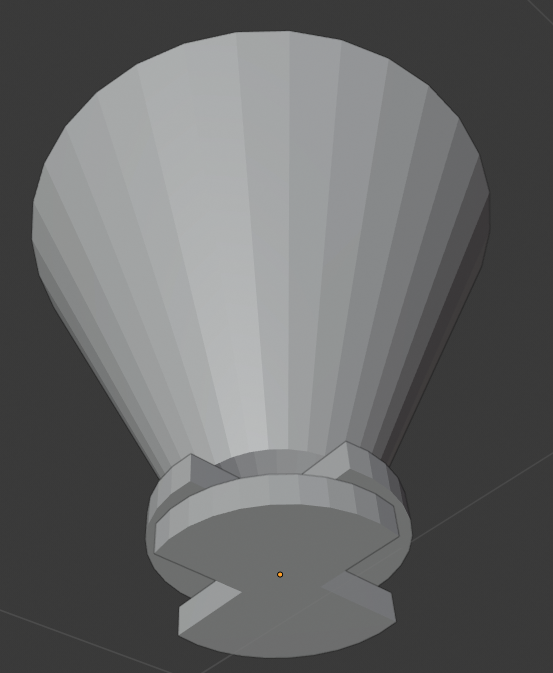
\includegraphics[width=\linewidth]{img/PlanB.PNG}
     \caption{Disks and Reservoir}
     \label{fig:Disk1}
     \end{subfigure}
     \begin{subfigure}[b]{0.49\linewidth}
     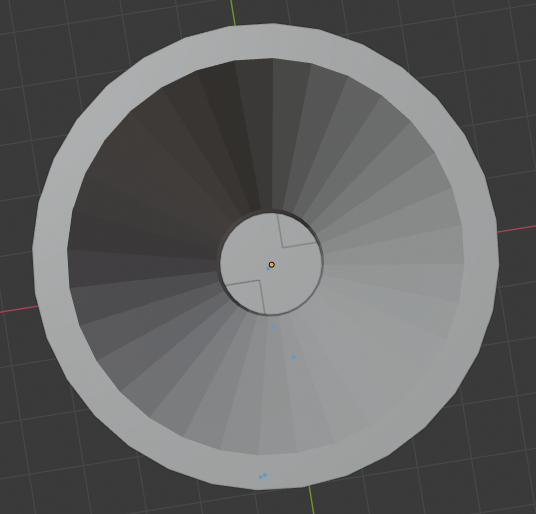
\includegraphics[width=\linewidth]{img/PlanB2.PNG}
     \caption {Disks and Reservoir in Off state}
     \label{fig:Disk2}
     \end{subfigure}
     \caption{The representation of the states of the cylinder}
     \label{fig:Disk}
\end{figure}

Both of these solutions require test which will be mentioned on the Test and Test Plans part. 

\subsubsection{Dog Deterring System}
Unwanted dogs must be removed from the area without giving harm to them. In order to solve this problem two different solution are considered.
\paragraph{Plan A}
Dogs can be removed from the area via using dazer. Dazers aim is to repel the dogs using 25.000 Hz signal\cite{cite:Dazer}. This frequency is far beyond a human to hear however dogs can hear this signal and leave the area. The problem of this device is that cats can also hear this frequency range and react to it. Therefore they can also leave. Moreover, dogs can get use to this voice and as time passes, dazer might not be an effective way to deter them.
\paragraph{Plan B}
Dogs can be deterred by squeezing water on them. The water must have a high pressure so that it will hurt the dog bot not harm it. However there exist several drawback of this plan since one will need an extra place in the box to store the water, which also will have a weight. Moreover, the user will be responsible for supplying water to the system. Most importantly for this system to be effective the box and dog should be close to each other so that dog can fear from pressure and leave.

The planned test can be seen under Test Plans.

\subsubsection{Exterior Design}
The outer box should be reliable since it might be exposed to an attack of an aggressive animal and it has to resist the outdoor conditions such as heat and cold. Therefore in order to observe and select the right material, the above tests will be conducted which can be seen under test plans section of this report.

\subsection{Tests}

% ===== Procedure and results of tests ===== %
\subsubsection{Food Mechanism}
\paragraph{Description of the Test for Plan A}
Test was conducted in order to observe the behaviour of the food flow when we use Plan A.

The purpose of this test is:
\begin{itemize}
    \item Determine the quantity of the average amount of the food poured. 
    \item Determine if there any food is jammed between reservoir and the cylinder. If there exist some, determine if they will harm to rotation or not.
    \item Determine if motor is capable of rotating without difficulty.
\end{itemize}

Procedure can be followed below.
\begin{itemize}
    \item Fully fill the reservoir with food.
    \item Observe the food flow in reservoir in off condition.
    \item Rotate the cylinder and observe the amount of food flow.
    \item While rotating observe the food flow from reservoir to the solid part of the cylinder.
    \item Observe if there exist any food jammed between the solid part of the cylinder and the reservoir. 
    \item Return the cylinder to its old position.
    \item Observe if the flow of the food is completely stopped. 
    \item Turn the cylinder again and observe the food flow again. Compare with the previous amount of food flowed.
    \item Repeat this process 10 times. 
\end{itemize}


% ===== Justification of requirements ===== %
\paragraph{Results of the Experiment}
It is observed that food flow is not fully controllable in every rotation. It sometimes pours more food than cat needs in one cycle. In 4 trials food flowed more than expected (40 gr on average). Only in 4 trials 10 gr of food is flowed on average, which is an acceptable weight and in 2 trials food flow is not stopped. The results for the first test is not good however with some improvements on the current placement of the reservoir and the cylinder situation can become a lot greater. In the test for Plan A, these improvements will be done and the results will be checked if it now satisfies the necessary conditions. 

The food is jammed between the reservoir and the cylinder however it is observed that it contains no danger to the rotation of the cylinder since the motor has enough torque in order to rotate the disk. 

It is observed that when the camera and motor are connected to the same raspberry-pi, the motor starts to falter although when the motor is not rotating. This is due to the soft pwm that raspberry-pi provides. In order to overcome this problem, the motor driver will be used since it provides a hard pwm.



%It is observed that the average food flow is 5 gr for each rotation. In this case for a normal cat, the cylinder has to rotate X times. The rotation process takes X seconds. Therefore our mechanical response is X*Y=XY seconds. 
%It is observed that food flow is completely stopped at the 92 trials where at 5 trials only the food jammed between the reservoir and cylinder is flowed at maximum 2 gr. At 3 trials the food on the cylinder is poured when there exist a solid blockage in between, however the food flow is stopped after averagely 3 seconds with maximum of 6 gr food flow, averagely 4 gr food. In conclusion we can trust this design since it contains \%7 error with the amount which is not considerable when we think about the food has to be given to ordinary cat.
%The food is jammed between the reservoir and the cylinder however it is observed that it contains no danger to the rotation of the cylinder since motor has enough torque in order to rotate the disk. 
%It is observed that when the camera and motor is connected to the same raspberry-pi, motor starts to falter although when motor is not rotating. This is due to the soft pwm that raspberry-pi provides. In order to overcome this problem, motor driver will be used since it provides a hard pwm. 
% ===== Comparison with alternative solutions ===== %

% ===== Error sources, their impact and ways to mitigate ===== %
\newpage
\subsection{Plans}

% ===== State names of responsible person/people ===== %
There exist several test plans in order to check the systems reliability and considering the different plans for different subsystems. The responsible person and the working schedule can be seen from the figure~\ref{fig:GanttChart for Mechanical Part}..
%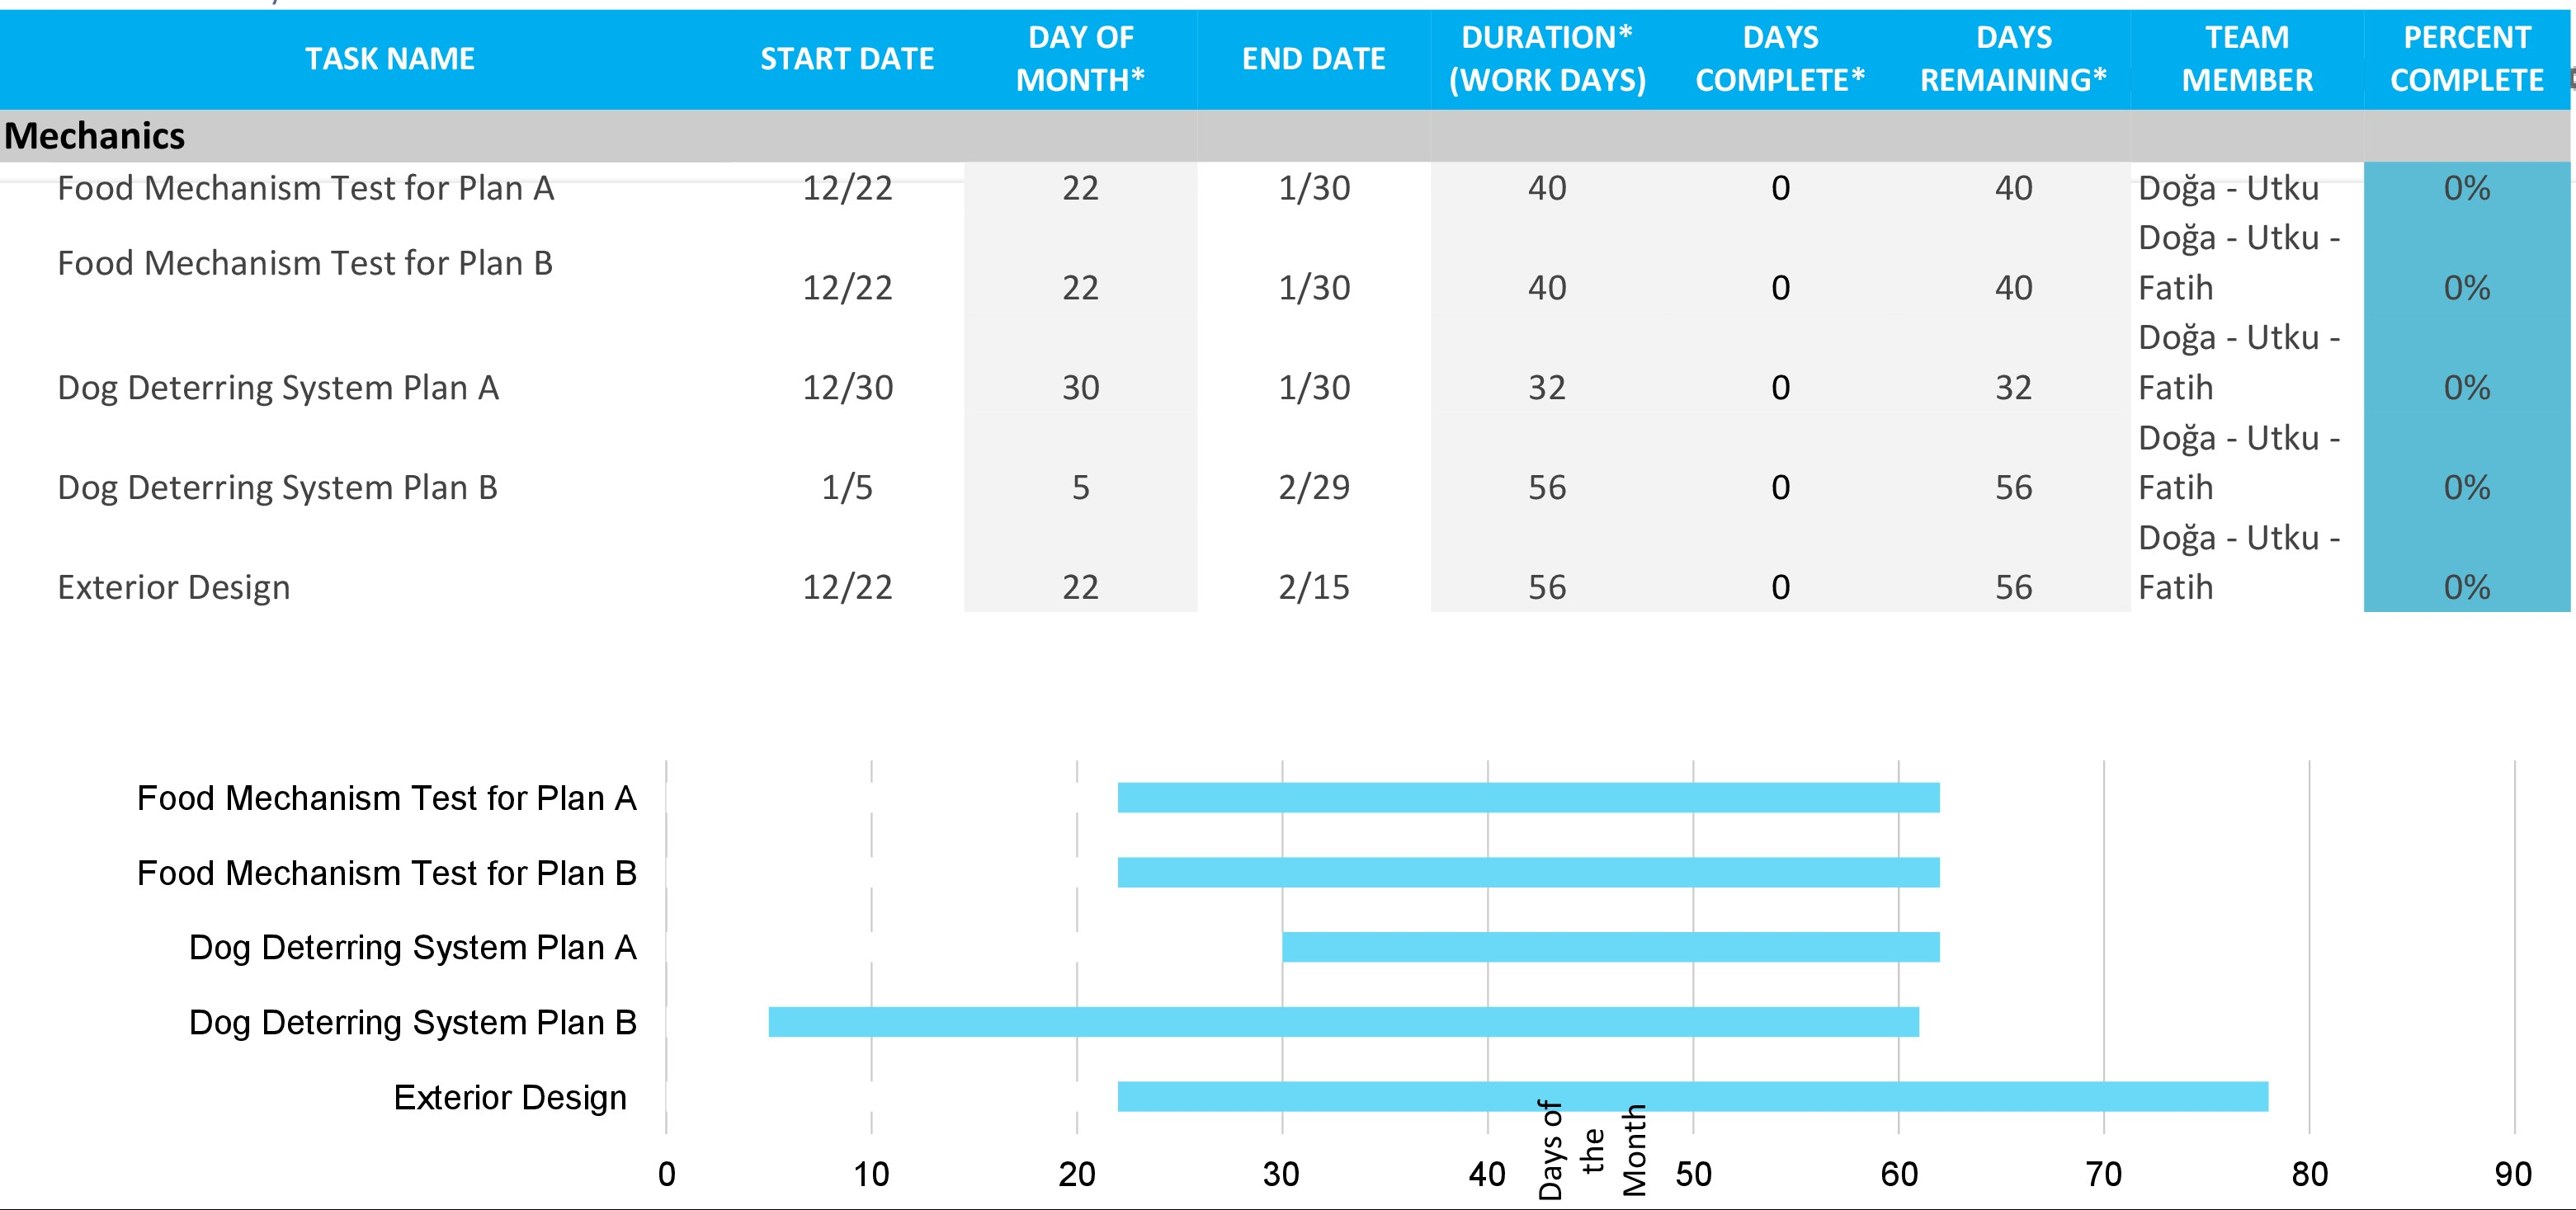
\includegraphics[width=15cm, height=10cm]{img/mekanikganttchart.jpg}
\begin{figure}[tbh]
    \centering
    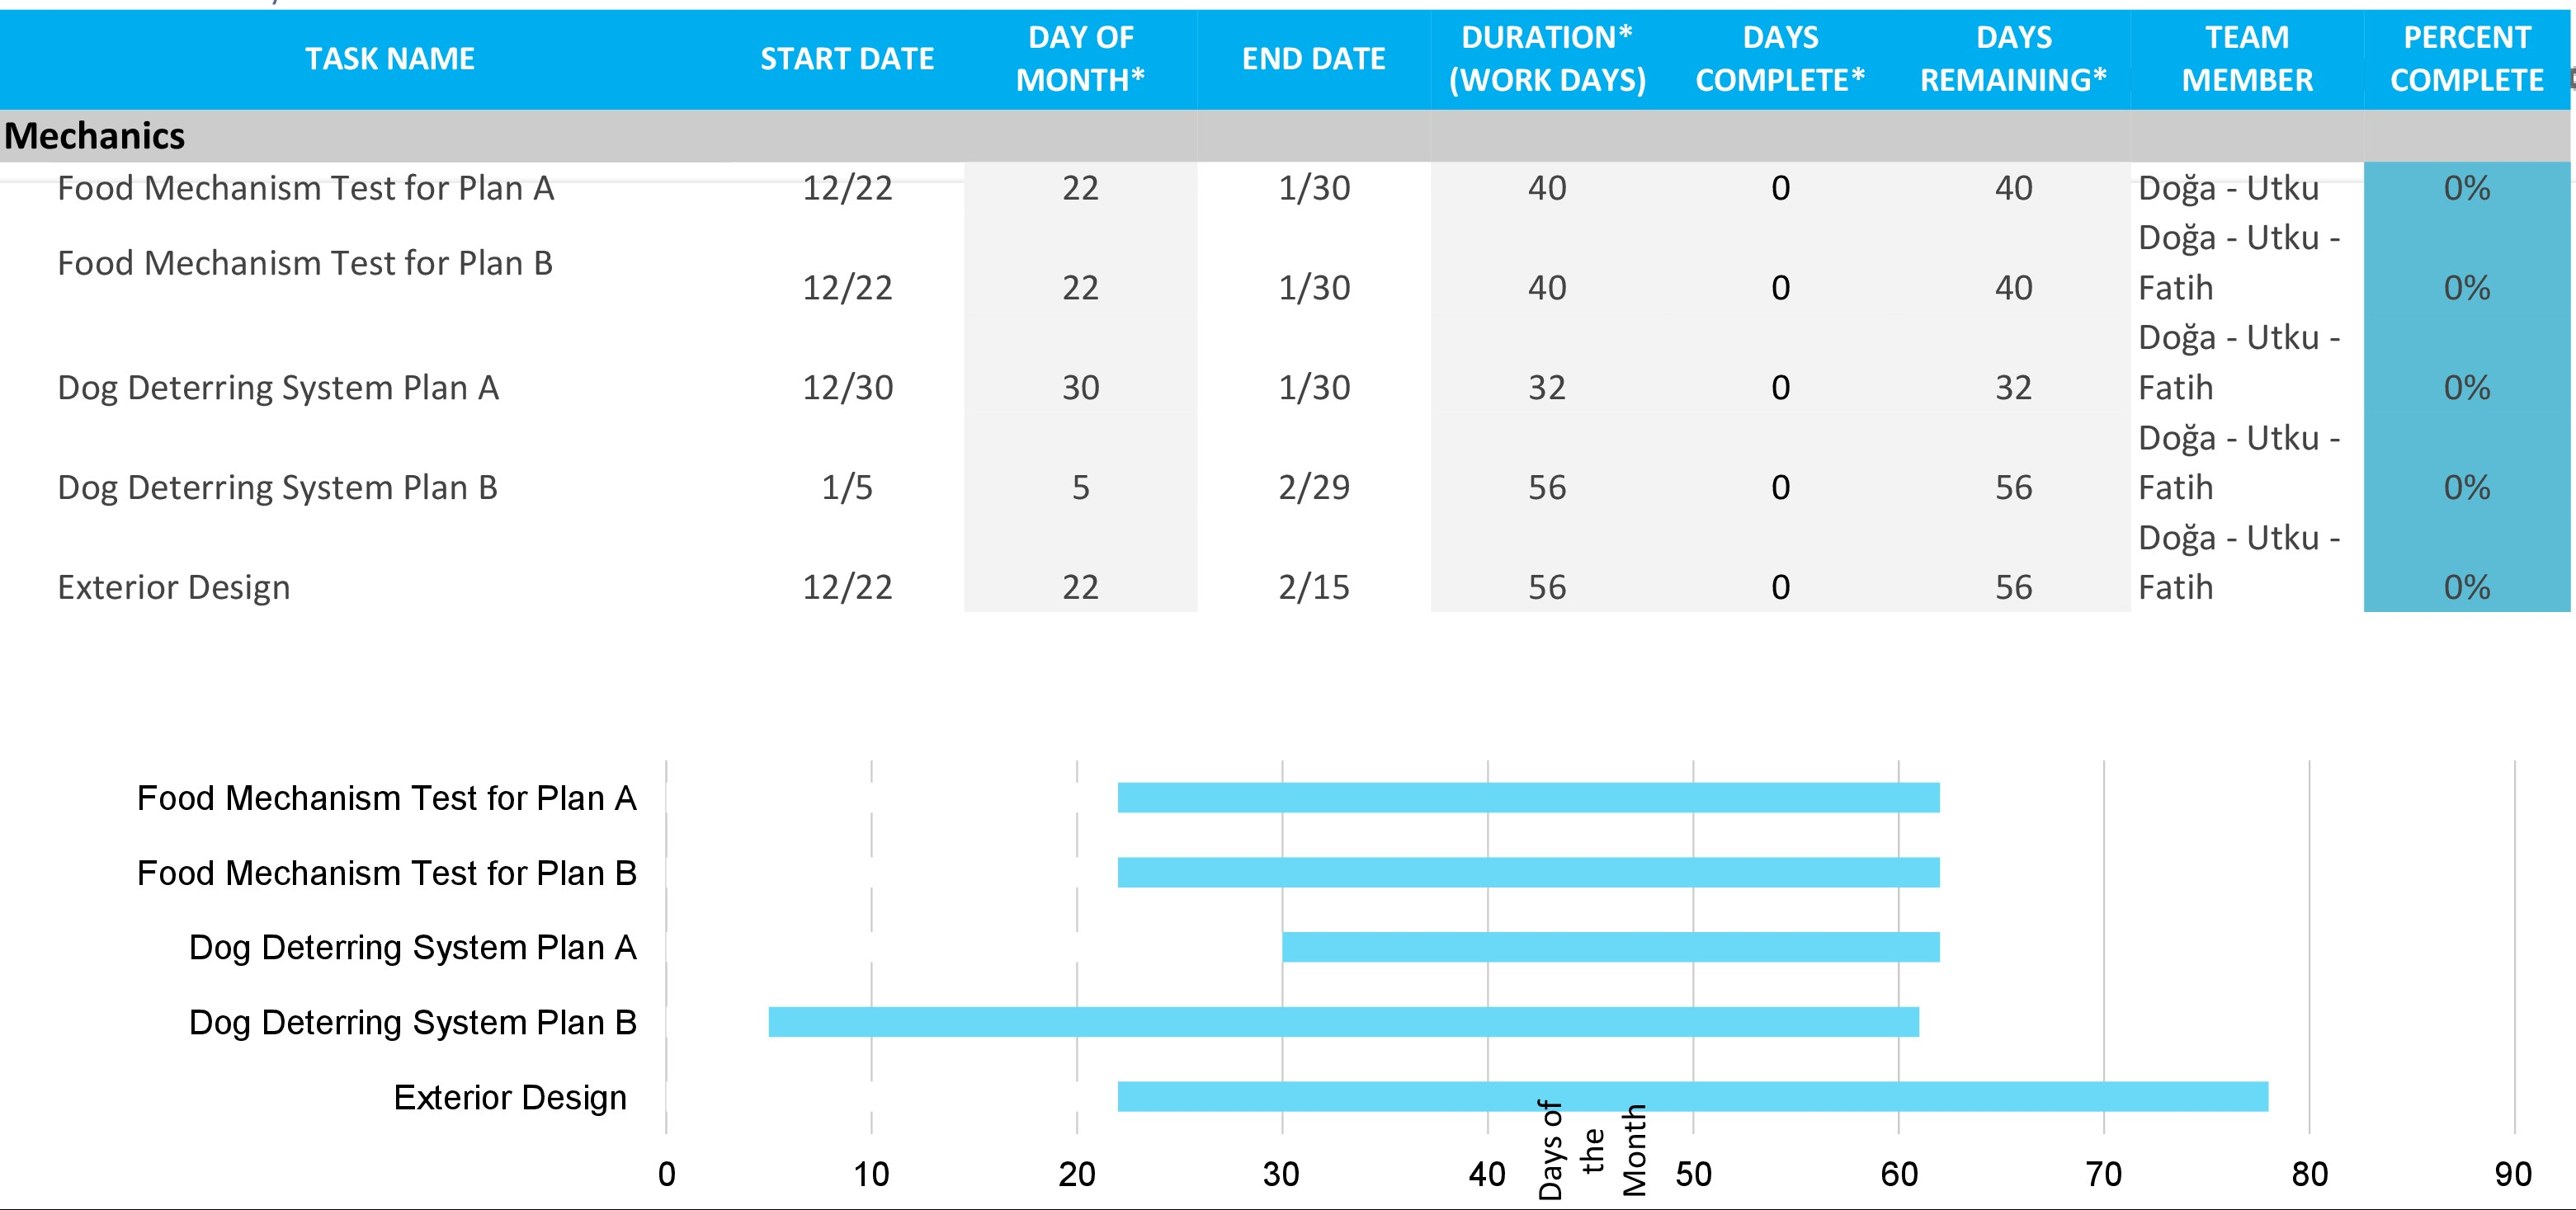
\includegraphics[width=15cm, height=10cm]{img/mekanikganttchart.jpg}
    \caption{Gantt Chart for Mechanical Part}
    \label{fig:GanttChart for Mechanical Part}
\end{figure}




\subsection{Anticipated Difficulties}
\subsubsection{Food Mechanism}
It is expected that the food mechanism will create problems in terms of controlling the amount of food flowed. In order to get over with lots of tests will be conducted until it satisfies the necessary conditions mentioned on the food mechanism part.
The balance of the cylinder and disk also might create an if a large amount of weight applies pressure on them but the first trials showed that, encountering this problem is a low probable one.
\subsubsection{Dog Deterring System}
Dogs are quite clever animals, therefore deterring them from the area by using the same method will create problems since they will understand that the precautions that taken will not harm them.

\subsection{Test Plans}
\subsubsection{Food Mechanism}
\paragraph{Plan A}
The same test procedure will be done, but only repeating 100 times via using a motor driver. The falter on the motor will be observed and the quantity of the food flow will be determined.
The measure of success for this experiment is to drive to the motor without being faltering. The successful stop rate for food flow is \%4 and the amount of food flow in every cycle should now vary \%10 in weight.

\paragraph{Plan B}
Purpose of this test is:
\begin{itemize}
    \item Determine the amount of the food flow according to the selected angled rotations. 
    \item Observe if there will be any jammed food between the disks, if there any observe if this will create a danger for controlling the quantity of the food. 
    \item Checking the reaction of the motor to an unstable load.
\end{itemize}

Procedure can be found below.
\begin{itemize}
    \item Fully fill the reservoir with food.
    \item Observe the food flow in reservoir in off condition.
    \item Rotate the disk to an certain angle and observe the amount of food flow.
    \item While rotating observe the food flow when one open and one solid parts of the disks match.
    \item Observe if there exist any food jammed between two disks.
    \item Return lower to its old position.
    \item Observe if the flow of the food is completely stopped. 
    \item Turn the disk again with a different angle and observe the food flow again. Compare with the previous amount of food flowed.
    \item Repeat this process for 4 different angle. 
    \item Determine the most efficient angle.
    \item Observe the quantity of the food flow for this efficient angle for 100 trials. 
\end{itemize}

% ===== Measure of success ===== %
The expected main problem is the reaction of the motor to an unstable load since, the load will be on one side of the disk, therefore it may create a shaking behaviour. The solution for this behavior can be cutting two sides which having the same axis. In this way one can solve the shaking problem, however, on the other hand, it might create a problem and controlling the amount of food flowing through.
The measure of success of this experiment is stopping the food flow at least 95 times, moreover, it is desired that the quantity of the food is also controllable. In each trial, one has to get a similar amount of food flow.

\subsubsection{Dog Deterring System}
There exist tow different tests for two different plans. Purpose of this tests are observing the response of dogs to the deterring system.
\paragraph{Plan A}
The procedure is:
\begin{itemize}
    \item Active the dazer system.
    \item Observe the behaviour of dogs when dazer is first applied.
    \item Observe the behaviour of cats.
    \item Repeat this process for 10 times.
    \item Observe the behaviour of the dogs after they get use to the sound of the dazer.
\end{itemize}
Measure of success of is achieving \%80 of deterring the dogs at first trial and \%60 of deterring when they get used to it. 

\paragraph{Plan B}
The procedure is:
\begin{itemize}
    \item Active the pressured water system.
    \item Observe the behaviour of the dog after it gets wet.
    \item Repeat this process 10 times with different dogs.
    \item Repeat same process 15 times with the same dog.
\end{itemize}
Measure of success of is achieving \%100 of deterring the dogs when they first encountered with the pressured water and \%80 when they used to it.  

\subsubsection{Exterior Design}
The purpose of test is to determine the reliability of the box.
\begin{itemize}
    \item Check the weight of the box. 
    \item Apply force on the box and check if there exist any considerable damage on it. If not continue.
    \item Place electronic devices and the food mechanism inside the box and apply for on the box. Check if electronic devices, camera and food mechanism works properly. Check the angle of the camera. Observe if it works functional. 
    \item Repeat this process 5 times.
\end{itemize}

The measure of success for this experiment is having non-considerable damage on the box and it is desired that all electronic devices and the food mechanism work as it was before applying force. Moreover, the camera can move a little but it is expected to capture photographs that can useful for identifying cats and dogs.